\documentclass[conference]{IEEEtran}
\usepackage[T1]{fontenc}
\usepackage{cite}
\usepackage{graphicx,amsmath,amssymb,booktabs,array,xurl}
\usepackage{tikz}
\usetikzlibrary{arrows.meta,positioning,calc}
\usepackage[hidelinks]{hyperref}
\graphicspath{{figures/}}
\makeatletter\newcommand{\gen}[1]{\@@input generated/#1 }\makeatother
\definecolor{gat}{HTML}{2A78D6}
\definecolor{gru}{HTML}{EB6834}
\definecolor{ink}{HTML}{52514E}
\definecolor{resp}{HTML}{6250D6}

\title{Graph-Attention Traffic Speed Forecasting\\and a Synthetic LWR Signal-Control Study}
\author{\IEEEauthorblockN{Kavya Katal, Rudraksh Sharma, Anshuman Mehta, Vridhi Chaudhary, Bineet Keshari}
\IEEEauthorblockA{Team T072, Section C, Rishihood University\\
Project 4, Phase 2 (Deep Learning) report, November 2026}}

\begin{document}
\maketitle

\begin{abstract}
In Phase 1 we predicted traffic speed on the METR-LA road sensors with one tree model per sensor. In Phase 2 we ask one deep-learning question: does a neural network forecast better when it can also look at neighbouring sensors on the road network? We train two small networks under the same rules. The first is a gated recurrent unit (GRU) that reads each sensor's own recent speeds. The second adds a graph-attention (GAT) layer that lets each sensor collect information from its neighbours. At 60 minutes ahead the GRU+GAT model has a mean absolute error (MAE) of 4.881\,mph. The same model with neighbours switched off has 4.931\,mph. Neighbours therefore help, but only by about 1\%. Both networks stay behind the Phase 1 XGBoost model (3.874\,mph), and a blend of XGBoost and GRU+GAT gives no gain. In a separate experiment we simulate a small road with the Lighthill--Whitham--Richards (LWR) traffic model and compare two rule-based signal agents with a fixed timetable. That simulation uses made-up traffic and is not connected to the forecasts. All forecasting scores are exploratory, because the test period was already inspected in Phase 1.
\end{abstract}

\begin{IEEEkeywords}
traffic forecasting, METR-LA, gated recurrent unit, graph attention network, ablation study, cell transmission model
\end{IEEEkeywords}

\section{Introduction}
Traffic speed at one place depends on two things: what happened there in the last few minutes, and what is happening on the roads connected to it. A queue grows backwards along a road, and released traffic moves forwards. A model that looks at one sensor alone cannot see the second effect.

Our Phase 1 models were of that kind. Random Forest and XGBoost each used 38 features built from a sensor's own last 55 minutes. Phase 2 tests whether a deep model that can also see neighbouring sensors does better. We designed the experiment so that any improvement can be traced to the neighbours and not to some other change.

The project title also mentions LWR traffic-flow models and multi-agent control. The dataset contains only speed, so these topics cannot be studied on the real data. We cover them with a small simulation, kept separate from the forecasting.

The work has three parts:
\begin{itemize}
\item \textbf{Forecasting models.} A GRU and a GRU with a graph-attention layer, trained with the same data rules as Phase 1 (Sections III--V).
\item \textbf{Controlled tests.} Three ablations and an ML--DL blend, to see what each part of the model contributes (Sections VI--VII).
\item \textbf{Simulation.} An eight-cell LWR road with two signal agents (Section VIII).
\end{itemize}

\section{Literature Review}
We read the sources below for ideas and methods. We did not reproduce their experiments, and we do not compare our scores with theirs, because their data splits and training procedures differ from ours. Table~\ref{tab:lit} summarises how each source is used.

\textbf{Learning from a sequence.} Cho \emph{et al.} introduced the gated recurrent unit \cite{cho}. It reads a sequence one step at a time and uses two gates to decide what to remember and what to overwrite. We use a GRU to summarise each sensor's recent speeds.

\textbf{Learning from a graph.} Veli\v{c}kovi\'c \emph{et al.} proposed graph attention networks \cite{gat}. Each node collects information from its neighbours and learns how much weight to give each one. Our graph layer follows this design.

\textbf{Traffic forecasting on a road graph.} Li \emph{et al.} combined a recurrent network with diffusion on a directed sensor graph (DCRNN) and released the METR-LA dataset and its road graph \cite{dcrnn}. We use their dataset and graph. Our model is much smaller and is not a copy of DCRNN.

\textbf{Traffic-flow theory.} Lighthill and Whitham \cite{lw} and Richards \cite{richards} described traffic as a fluid in which vehicles are conserved. This is the LWR model. Daganzo turned it into a simple computation, the cell transmission model (CTM), by cutting the road into cells \cite{ctm}. We implemented the update as described in a Berkeley technical overview \cite{ctmoverview}.

\textbf{Signal control.} Lioris and Varaiya study max-pressure control, in which each junction serves the approach with the largest difference between waiting vehicles upstream and downstream, using only local measurements \cite{lioris}. Our responsive signal agent borrows this idea in a simplified form and claims none of its theoretical guarantees.

\textbf{The machine-learning baseline.} Chen and Guestrin's XGBoost builds an ensemble of decision trees, each correcting the errors of the previous ones \cite{xgb}. It was our best Phase 1 model. In Phase 2 it is the model the networks are compared with, and the ML half of our hybrid.

\begin{table*}[t]\centering\small
\caption{Sources and how this project uses them.}\label{tab:lit}
\begin{tabular}{@{}p{0.2\textwidth}p{0.37\textwidth}p{0.37\textwidth}@{}}\toprule
Source & Main idea & Use in this project\\\midrule
GRU \cite{cho} & A recurrent unit with reset and update gates & Summarises each sensor's last 12 readings\\
GAT \cite{gat} & A node weighs its neighbours with learned attention & Lets a sensor use its road-graph neighbours\\
DCRNN \cite{dcrnn} & Recurrent forecasting on a directed road graph & Source of the dataset and the sensor graph\\
LWR \cite{lw,richards} & Vehicles are conserved; flow depends on density & Theory behind the simulation\\
CTM \cite{ctm,ctmoverview} & LWR computed on road cells with send and receive limits & The simulation update rule\\
Max pressure \cite{lioris} & Serve the approach with the highest local pressure & Idea behind the responsive signal agent\\
XGBoost \cite{xgb} & Boosted ensemble of decision trees & Best Phase 1 model; ML half of the hybrid\\
\bottomrule\end{tabular}
\end{table*}

\section{Dataset and Preparation}
\textbf{Dataset.} METR-LA has speed readings from 207 loop sensors on Los Angeles highways, taken every five minutes from 1 March to 27 June 2012 \cite{dcrnn}. That gives 34,272 time steps. Speeds are in miles per hour. A missing reading is stored as zero; 8.11\% of all readings are missing. The road graph that comes with the dataset has 1,515 directed links between sensors.

\textbf{Task.} The model sees the last 12 readings of every sensor (55 minutes) and predicts the next 12 (5 to 60 minutes ahead). We report results at 15, 30 and 60 minutes.

\textbf{Splitting by time.} The data are split in time order, never randomly: 23,963 forecast points for training, 1,701 for tuning, 1,702 kept aside for the blend, and 6,850 for testing. Eleven points are dropped before each boundary so that no answer from one part falls inside the next part.

\textbf{Avoiding leakage.} Leakage means that information from the future, or from the test data, slips into training. We prevent it in three ways.
\begin{itemize}
\item Every statistic (the mean and spread used for scaling, and one median per sensor) is computed from training readings only.
\item A missing input is filled from an earlier reading in the same window, or from the sensor's training median. Inputs are never filled from later readings.
\item A missing answer is never filled. It is left out of the loss and of every score, for all methods alike.
\end{itemize}

\textbf{Inputs.} For each sensor and time step the network receives two numbers: the scaled speed and a flag saying whether the reading was missing. It also receives five calendar values (time of day and day of week as sine and cosine, and a weekend flag).

\section{Model}
\begin{figure*}[t]
\centering
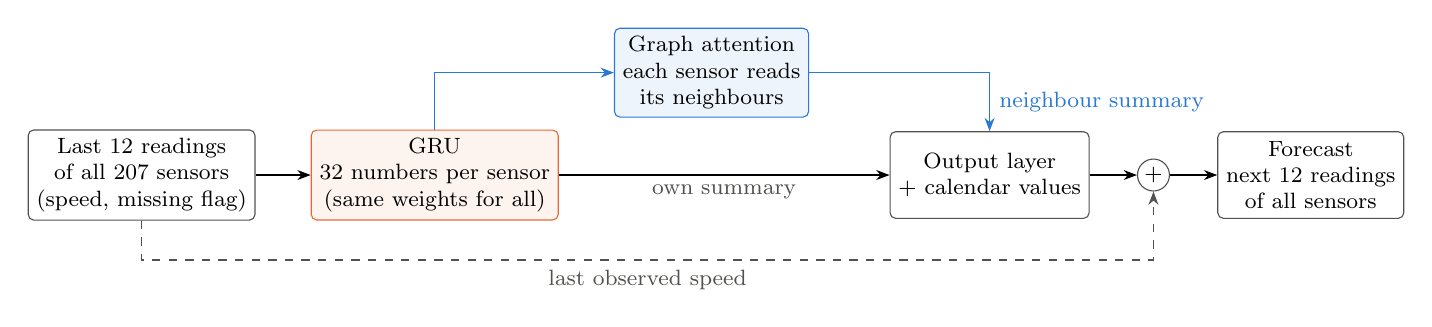
\begin{tikzpicture}[font=\footnotesize, >=Stealth,
  box/.style={draw=ink, rounded corners=2pt, align=center, minimum height=11mm, inner sep=3pt, fill=white},
  gbox/.style={box, draw=gat, fill=gat!8},
  ebox/.style={box, draw=gru, fill=gru!8}]
\node[box] (in) {Last 12 readings\\of all 207 sensors\\(speed, missing flag)};
\node[ebox, right=7mm of in] (gru) {GRU\\32 numbers per sensor\\(same weights for all)};
\node[gbox, right=7mm of gru, yshift=13mm] (gat) {Graph attention\\each sensor reads\\its neighbours};
\node[box, right=42mm of gru] (head) {Output layer\\+ calendar values};
\node[circle, draw=ink, inner sep=1pt, right=6mm of head] (sum) {$+$};
\node[box, right=6mm of sum] (out) {Forecast\\next 12 readings\\of all sensors};
\draw[->] (in) -- (gru);
\draw[->] (gru) -- node[below, text=ink]{own summary} (head);
\draw[->, gat] (gru.north) |- (gat.west);
\draw[->, gat] (gat.east) -| node[pos=0.75, right, text=gat]{neighbour summary} (head.north);
\draw[->] (head) -- (sum);
\draw[->] (sum) -- (out);
\draw[->, ink, dashed] (in.south) -- ++(0,-5mm) -| node[pos=0.25, below, text=ink]{last observed speed} (sum.south);
\end{tikzpicture}
\caption{The two models. The temporal GRU uses the black path only. GRU+GAT adds the blue branch. The network predicts a correction that is added to the last observed speed.}
\label{fig:arch}
\end{figure*}

Fig.~\ref{fig:arch} shows both models. They are identical except for the blue branch.

\subsection{GRU: reading one sensor's history}
A GRU reads the 12 readings of a sensor one by one and keeps a memory $h_t$ of 32 numbers. At each step, with input $x_t$,
\begin{align}
r_t&=\sigma(W_r x_t+U_r h_{t-1}+b_r),\\
z_t&=\sigma(W_z x_t+U_z h_{t-1}+b_z),\\
n_t&=\tanh\bigl(W_n x_t+b_n+r_t\odot(U_n h_{t-1}+c_n)\bigr),\\
h_t&=(1-z_t)\odot n_t+z_t\odot h_{t-1}.
\end{align}
Here $\sigma$ is the sigmoid function, which gives values between 0 and 1, and $\odot$ multiplies element by element \cite{cho}. In words: $n_t$ is a proposed new memory. The reset gate $r_t$ decides how much of the old memory is used to form that proposal. The update gate $z_t$ decides how much of the old memory is kept and how much is replaced. After 12 steps the memory $h_i$ is a summary of sensor $i$. One GRU, with one set of weights, is used for all 207 sensors.

\subsection{Graph attention: listening to neighbours}
The graph model passes the 207 summaries through one attention layer \cite{gat}. For sensor $i$ and a neighbour $j$,
\begin{align}
e_{ij}&=\operatorname{LeakyReLU}\bigl(a_r^{\top}Wh_i+a_s^{\top}Wh_j\bigr),\\
\alpha_{ij}&=\frac{\exp(e_{ij})}{\sum_{k\in\mathcal N_i}\exp(e_{ik})},\\
g_i&=\operatorname{ELU}\Bigl(\sum_{j\in\mathcal N_i}\alpha_{ij}\,Wh_j\Bigr).
\end{align}
The score $e_{ij}$ says how useful neighbour $j$ looks to sensor $i$. The second line turns the scores into weights $\alpha_{ij}$ that are positive and add up to one. The third line is a weighted average of the neighbours' summaries. The set $\mathcal N_i$ contains sensor $i$ itself and the sensors with a road-graph link into $i$. The graph only decides who counts as a neighbour; the weights are learned. We use two such attention heads of 16 numbers each and join their outputs.

\subsection{Output: a correction to the last speed}
The output layer takes the sensor's own summary, the neighbour summary (graph model only) and the calendar values, and produces 12 numbers. These are added to the sensor's last observed speed:
\begin{equation}
\hat y_{i}=\text{last speed}_i+W_o\,[h_i;g_i;c_t]+b_o .
\end{equation}
The output weights start at zero. An untrained model therefore predicts ``the speed stays as it is'', which is the persistence forecast, and training only has to learn how to improve on that.

\subsection{Why the model is small}
The temporal GRU has 3,912 parameters and GRU+GAT has 5,384. A small model trains in roughly 15 to 25 minutes on a laptop CPU. This let us repeat training with three random seeds and run several ablations, and it keeps the comparison between variants clean. The price is accuracy, as Section VII shows.

\section{Training and Regularisation}
The loss is the mean absolute error over the answers that are not missing. Table~\ref{tab:hyper} lists the settings. They were written into a configuration file before any training on real data.

\begin{table}[t]\centering\small
\caption{Training settings, fixed before training.}\label{tab:hyper}
\begin{tabular}{@{}ll@{}}\toprule
Setting & Value\\\midrule
Input / output length & 12 / 12 steps (5\,min each)\\
GRU memory size & 32, one layer\\
Attention & 2 heads $\times$ 16 numbers\\
Loss & masked mean absolute error\\
Optimiser & Adam, weight decay $10^{-4}$\\
Learning rates tried & $10^{-3}$ (chosen), $3\times10^{-4}$\\
Batch size & 32 forecast points\\
Dropout & 0.1\\
Gradient clipping & norm 5\\
Epochs & at most 50; stop after 7 without gain\\
Random seeds & 42, 43, 44\\
\bottomrule\end{tabular}
\end{table}

Regularisation means methods that stop a model from memorising its training data. We use four.
\begin{itemize}
\item \emph{Dropout}: during training, 10\% of the values in the sensor summaries and attention weights are randomly set to zero.
\item \emph{Weight decay}: a small penalty on large weights.
\item \emph{Gradient clipping}: very large update steps are scaled down, which keeps recurrent training stable.
\item \emph{Early stopping}: training ends when the error on the tuning data has not improved for seven epochs, and the best version is kept.
\end{itemize}
Sharing one GRU across all sensors also limits over-fitting, because the same weights must work for every road.

We tried two learning rates for each model and kept the one with the lower error on the tuning data: $10^{-3}$ in both cases (tuning MAE 3.335\,mph for the GRU and 3.306\,mph for GRU+GAT). No setting was chosen using test scores.

\section{Experiments}
\textbf{Methods compared.} Four Phase 1 methods serve as references: persistence (the speed stays as it is), historical average (the usual speed for that sensor and time of week), Random Forest and XGBoost. Their saved predictions are scored again on exactly the same answers as the neural models.

\textbf{Ablations.} An ablation removes one part of a model to see how much that part matters. We run three, each changing one thing in GRU+GAT:
\begin{itemize}
\item \emph{Self-loop only}: every sensor may look only at itself. The attention layer and its parameters stay. Only the neighbours are removed.
\item \emph{Uniform neighbours}: neighbours are averaged with equal weights, so the learned weighting is removed.
\item \emph{No dropout}: dropout is switched off.
\end{itemize}
The temporal GRU also has no neighbours, but it is a smaller model. The self-loop model has the same size as GRU+GAT, so it is the fair test of what neighbours add. The two main models and the self-loop model are trained with three seeds; the other two ablations with one.

\textbf{Hybrid approach.} Phase 2 allows a hybrid that combines an ML model with a DL model. Ours combines the best Phase 1 model with the graph network by a weighted average:
\[\hat y=\lambda\,\hat y_{\mathrm{XGB}}+(1-\lambda)\,\hat y_{\mathrm{GAT}},\qquad \lambda\in\{0,\,0.25,\,0.5,\,0.75,\,1\}.\]
\emph{Why it could help.} The two models learn in different ways. XGBoost has a separate model for every sensor and sees only that sensor. The network shares its weights across sensors and sees the neighbours. Models that differ like this often make different mistakes, and averaging can cancel some of them.

\emph{How we keep it fair.} The weight $\lambda$ is chosen on 1,702 forecast points that were kept aside and used for nothing else. It is fixed before the test data are scored. The two pure models ($\lambda=0$ and $\lambda=1$) are among the candidates, so the procedure can also tell us that blending does not help.

\textbf{Scores.} With error $e_j$ on each of the $n$ scored answers,
\[\mathrm{MAE}=\frac1n\sum_j|e_j|,\qquad \mathrm{RMSE}=\sqrt{\frac1n\sum_j e_j^2}.\]
Both are in mph and lower is better. MAE is the typical size of an error. RMSE punishes large errors more. Each horizon has about 1.25 million scored answers.

\section{Results}
\begin{table*}[t]\centering\small
\caption{Test error in mph. Neural rows are the mean $\pm$ standard deviation over three training runs with different seeds. Phase 1 rows are single saved runs. Bold marks the best value in each column.}\label{tab:main}
\begin{tabular}{@{}lrrrrrr@{}}\toprule
Method & MAE 15\,min & MAE 30\,min & MAE 60\,min & RMSE 15\,min & RMSE 30\,min & RMSE 60\,min\\\midrule
\gen{table_main.tex}
\bottomrule\end{tabular}
\end{table*}

\begin{figure}[t]\centering
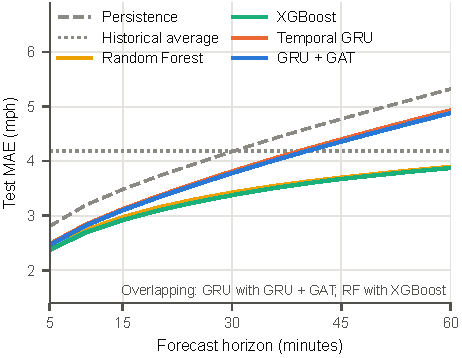
\includegraphics[width=\columnwidth]{horizons.pdf}
\caption{Test MAE at every forecast horizon from 5 to 60 minutes.}\label{fig:horizons}
\end{figure}

\subsection{How the models compare}
Table~\ref{tab:main} and Fig.~\ref{fig:horizons} show three things.

\emph{The networks beat persistence.} GRU+GAT has 11.0\% less error than persistence at 15 minutes and 8.3\% less at 60 minutes.

\emph{The tree models are better.} XGBoost has the lowest MAE at all three horizons and Random Forest the lowest RMSE. At 60 minutes GRU+GAT is 1.007\,mph behind XGBoost.

\emph{At long horizons the networks lose even to the historical average.} From 45 minutes onward (40 for the temporal GRU), the historical average of 4.187\,mph is better than both networks. Far ahead, the usual speed for that time of the week is a better guide than the latest reading, and our networks do not move far enough from the latest reading.

A likely reason for the gap to the tree models, which we did not test, is this. Phase 1 trains a separate model for every sensor, so each model can learn the daily pattern of its own road. Our network uses one small set of weights for all 207 sensors and is not told which sensor it is looking at.

\subsection{Do neighbours help?}
\begin{table}[t]\centering\small
\caption{Ablations: test MAE in mph. The last column is the change at 60\,min against the full model; a positive value means worse.}\label{tab:abl}
\setlength{\tabcolsep}{3.5pt}
\begin{tabular}{@{}lrrrr@{}}\toprule
Variant & 15\,min & 30\,min & 60\,min & Change\\\midrule
\multicolumn{5}{@{}l}{\emph{Seed 42}}\\
\gen{table_ablation.tex}
\bottomrule\end{tabular}
\end{table}

\begin{figure}[t]\centering
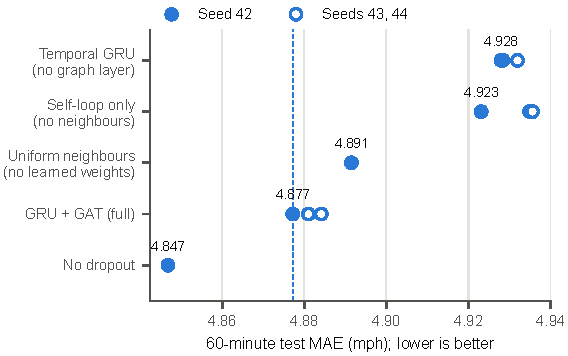
\includegraphics[width=\columnwidth]{ablation.pdf}
\caption{60-minute test MAE of every trained variant. Each circle is one training run. The whole axis covers only 0.09\,mph.}\label{fig:abl}
\end{figure}

Yes, slightly. Averaged over three seeds, the full model has a 60-minute MAE of 4.881\,mph and the self-loop model 4.931\,mph (Table~\ref{tab:abl}). The difference is 0.050\,mph, about 1\%. It appears in all three seeds (Fig.~\ref{fig:abl}) and it grows with the horizon, from 0.011\,mph at 5 minutes to 0.050\,mph at 60 minutes. Three seeds show how much results vary between runs. They are not a statistical significance test.

The other comparisons add detail.
\begin{itemize}
\item The self-loop model and the temporal GRU score almost the same (4.931 and 4.929\,mph). The extra layer alone brings nothing; the gain comes from the neighbours.
\item With equal weights the error is 4.891\,mph. Most of the gain is already there with a plain average of the neighbours; learning the weights adds 0.014\,mph (one seed).
\item Without dropout the error is 4.847\,mph, which is better. A model this small does not over-fit, so dropout was not needed. We kept the setting we had fixed in advance and did not retune after seeing a test result (one seed).
\item Looking at sensors one by one (seed 42), the full model is better than the self-loop model at 168 of 207 sensors.
\end{itemize}
Every method is much worse in rush hours. For GRU+GAT the 60-minute MAE is 7.691\,mph in peak periods and 4.174\,mph outside them.

\subsection{Hybrid result}
\begin{table}[t]\centering\small
\caption{Choosing the blend weight on the data kept aside. MAE is the mean over 15, 30 and 60 minutes, in mph.}\label{tab:hybrid}
\begin{tabular}{@{}rrrc@{}}\toprule
XGBoost share $\lambda$ & GAT share & MAE & Chosen\\\midrule
\gen{table_hybrid.tex}
\bottomrule\end{tabular}
\end{table}
The error falls with every step towards XGBoost, and the best weight is $\lambda=1$ (Table~\ref{tab:hybrid}). The chosen ``blend'' is therefore XGBoost alone, and its test error is the XGBoost row of Table~\ref{tab:main}.

The hybrid was built and tested as planned, but it showed no benefit. A blend helps when its parts are about equally good. Here the graph network is about 1\,mph worse than XGBoost, so mixing it in only raises the error. We do not claim a hybrid improvement.

A stronger hybrid, which we did not build, would let the two models work together instead of averaging them: for example, the network could be trained to predict the errors that XGBoost makes, or could take XGBoost's forecast as an extra input.

\section{Synthetic LWR Study with Two Signal Agents}
This section is a separate experiment. METR-LA has speed only, with no vehicle counts, densities or signal timings, so a traffic-flow model cannot be fitted to it. The simulation below uses assumed road parameters and invented demand. Its results say nothing about Los Angeles.

\subsection{The traffic model}
The LWR model says that vehicles are neither created nor lost along a road \cite{lw,richards}:
\begin{equation}
\frac{\partial\rho}{\partial t}+\frac{\partial q}{\partial x}=0,\qquad q=\rho v,
\end{equation}
where $\rho$ is density (vehicles per km), $q$ is flow (vehicles per hour) and $v$ is speed. We assume a free speed $v_f$ of 60\,km/h, a jam density $\rho_J$ of 150 vehicles per km and a backward wave speed $w$ of 20\,km/h. These give a road capacity $Q$ of 2250 vehicles per hour.

The cell transmission model \cite{ctm,ctmoverview} computes this on a road cut into cells. In each time step a cell can send only the vehicles it holds, and receive only as many as it has room for:
\begin{align}
\text{send}_i&=\min(v_f\rho_i,\;Q),\\
\text{receive}_i&=\min\bigl(Q,\;w(\rho_J-\rho_i)\bigr),\\
\text{flow}_{i\to j}&=\min(\text{send}_i,\ \text{receive}_j)\ \text{ on green, } 0\text{ on red}.
\end{align}
Each cell's content then changes by what flowed in minus what flowed out. Our cells are 250\,m long and a step is 5 seconds. A vehicle at free speed covers 83\,m in one step, less than a cell. This is the stability rule known as the CFL condition, and the code refuses settings that break it.

\begin{figure}[t]\centering
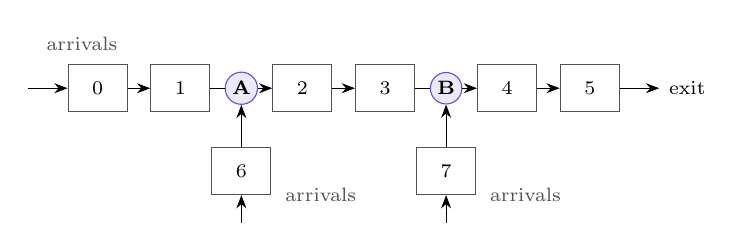
\begin{tikzpicture}[font=\scriptsize, >=Stealth,
  cell/.style={draw=ink, minimum width=7.5mm, minimum height=6mm, inner sep=0pt},
  sig/.style={circle, draw=resp, fill=resp!12, inner sep=1.2pt, font=\scriptsize\bfseries}]
\foreach \i/\x in {0/0,1/1.05,2/2.6,3/3.65,4/5.2,5/6.25} \node[cell] (c\i) at (\x,0) {\i};
\foreach \i/\j in {0/1,2/3,4/5} \draw[->] (c\i) -- (c\j);
\node[sig] (A) at ($(c1)!0.5!(c2)$) {A};
\node[sig] (B) at ($(c3)!0.5!(c4)$) {B};
\draw (c1) -- (A); \draw[->] (A) -- (c2);
\draw (c3) -- (B); \draw[->] (B) -- (c4);
\node[cell] (c6) at ($(A)+(0,-1.05)$) {6};
\node[cell] (c7) at ($(B)+(0,-1.05)$) {7};
\draw[->] (c6) -- (A); \draw[->] (c7) -- (B);
\draw[->] ($(c0.west)+(-5mm,0)$) -- (c0.west);
\draw[->] ($(c6.south)+(0,-3.5mm)$) -- (c6.south);
\draw[->] ($(c7.south)+(0,-3.5mm)$) -- (c7.south);
\draw[->] (c5.east) -- ++(5mm,0) node[right]{exit};
\node[anchor=south, text=ink] at ($(c0.north)+(-2mm,0.5mm)$) {arrivals};
\node[anchor=west, text=ink] at ($(c6.east)+(0.5mm,-3mm)$) {arrivals};
\node[anchor=west, text=ink] at ($(c7.east)+(0.5mm,-3mm)$) {arrivals};
\end{tikzpicture}
\caption{The simulated road: main cells 0 to 5 and side cells 6 and 7. Signal agent A lets either cell 1 or cell 6 enter cell 2. Agent B lets either cell 3 or cell 7 enter cell 4.}\label{fig:corridor}
\end{figure}

\subsection{The road and the two agents}
Fig.~\ref{fig:corridor} shows the road. Vehicles that cannot enter a full cell wait in a queue at the entrance, so none is lost. Each agent gives green to one of two approaches; between two greens there is a 5-second all-red pause.

The \emph{fixed-time} agents follow a timetable: 40\,s green for the main road, 5\,s all-red, 40\,s green for the side road, 5\,s all-red. They ignore traffic.

The \emph{responsive} agents look only at their own junction. For each approach an agent computes a pressure: the number of vehicles on the approach minus the number in the cell after the junction. After at least 20\,s of green it switches if the other approach has more pressure by over two vehicles, or if its own approach is empty while the other is not. It must switch after 60\,s. This follows the local-pressure idea of \cite{lioris} in a simplified form.

Both kinds of agent are written by hand as rules. Nothing is trained, so this is not reinforcement learning. The two agents send no messages to each other; they affect each other only through the traffic between them. No forecast from the neural models enters a signal decision.

\subsection{Experiment and results}
We defined four demand patterns before running anything: balanced demand, a main-road peak, a side-road peak and a temporary limit at the exit. Each has 60 minutes of arrivals and 20 minutes to drain. With five random seeds this gives 20 cases, and both kinds of agent receive exactly the same arrivals in each case: 40 runs in total.

\begin{table*}[t]\centering\small
\caption{Simulation results, mean over five seeds, in vehicle-minutes. System time counts every vehicle on the road or queued at an entrance. Entrance wait counts the queued ones only. These are simulation outputs, not measurements from Los Angeles.}\label{tab:control}
\begin{tabular}{@{}lrrrrr@{}}\toprule
 & \multicolumn{3}{c}{System time} & \multicolumn{2}{c}{Entrance wait}\\\cmidrule(lr){2-4}\cmidrule(l){5-6}
Demand pattern & Fixed time & Responsive & Reduction (\%) & Fixed time & Responsive\\\midrule
\gen{table_control.tex}
\bottomrule\end{tabular}
\end{table*}

\begin{figure}[t]\centering
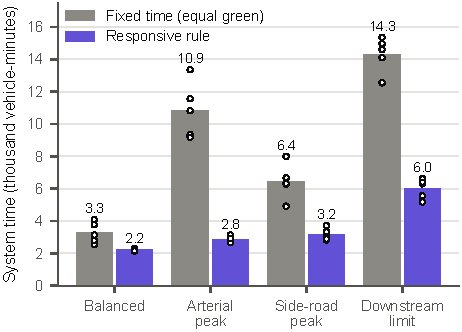
\includegraphics[width=\columnwidth]{control_bars.pdf}
\caption{System time for each demand pattern. Bars are means; circles are the five seeds.}\label{fig:bars}
\end{figure}

The responsive agents gave a lower system time in all 20 cases (Table~\ref{tab:control}, Fig.~\ref{fig:bars}). The size of the gap needs a careful reading. Under the fixed timetable each approach has green for 40 of every 90 seconds, so it can pass at most $2250\times40/90=1000$ vehicles per hour. The main-road peak sends 1100 per hour, so the fixed timetable cannot keep up and its queue keeps growing. A timetable with a longer main green would do far better. Ours was a simple equal split.

In all 40 runs the vehicle count balanced to within $3\times10^{-12}$ vehicles and no cell exceeded its jam density. Under the exit limit, the fixed timetable still had about four vehicles on the road when the simulation ended; they are kept in the totals.

The experiment shows that the traffic model conserves vehicles, that queues spill backwards, and that two local agents can work on the same road. It does not show a benefit in a real city, an optimal controller, multi-agent reinforcement learning, or control driven by our forecasts.

\section{Validation}
\begin{itemize}
\item \emph{Rules fixed first.} The experiment plan and all settings were recorded before training on real data.
\item \emph{Same answers for every method.} All methods are scored on identical targets. The re-scored Phase 1 predictions reproduce all 720 recorded Phase 1 scores.
\item \emph{Automated tests.} The repository has 76 tests. They check that no future data enters the inputs, that statistics come from training data only, that missing answers are ignored, the direction of the graph links, model shapes, saved-model loading, and the physics of the simulation. All 76 pass with the dataset present (run on 18 November 2026).
\item \emph{Repeatable results.} Each of the eleven saved models gives exactly the same predictions after reloading. The simulation always gives the same output; independent re-runs matched the saved results byte for byte.
\item \emph{One recorded change.} During the study the training machine ran short of memory, so input windows were built batch by batch and no longer stored all at once. All 34,249 windows were checked to be identical, and the model, data and scores were unaffected.
\end{itemize}

\section{Limitations}
\begin{itemize}
\item The test period was inspected in Phase 1. All forecasting scores are therefore exploratory, not a clean final estimate.
\item The neural models did not beat the tree models. They are small, were tuned over two learning rates only, and see 55 minutes of history.
\item Two ablations (uniform weights and no dropout) were run with one seed.
\item The data cover one city and four months. The time zone of the timestamps is not recorded.
\item Attention weights describe what the model learned. They do not prove how congestion moves between roads.
\item The simulation is a toy: assumed parameters, eight cells, no turning or lane changes, and a baseline that was not tuned to demand.
\item No project-specific brief beyond the general course instructions was available, so splitting the title into a forecasting part and a simulation part is our own reading.
\end{itemize}

\section{Conclusion}
Letting a small recurrent network see its road-graph neighbours lowered the 60-minute error from 4.931 to 4.881\,mph. A same-size model without neighbours shows that the neighbours are the reason. The gain is about 1\% and most of it comes from a plain average of the neighbours. It does not close the 1\,mph gap to XGBoost, and blending the two models gives no gain. On this dataset, and at this model size, one tree model per sensor is the better forecaster.

Separately, an LWR cell simulation conserved vehicles exactly and showed two local rule-based agents outperforming an equal-split timetable, mainly because that timetable was too weak for the main road.

Useful next steps are to tell the network which sensor it is looking at, to give it a longer history, to test on a period nobody has seen, and, if density or flow data become available, to fit the simulation to real roads.

\section*{Team Contributions and Assistance}
Kavya Katal coordinated the work. The Phase 2 code, experiments and saved results were prepared under that coordination with substantial AI assistance, building on the teammate prototype and the Phase 1 work. Each member integrated and reviewed one module through a pull request:

\smallskip
{\centering\small
\begin{tabular}{@{}p{0.27\columnwidth}p{0.67\columnwidth}@{}}\toprule
Member & Module\\\midrule
Vridhi Chaudhary & Data preparation for the networks and its tests\\
Bineet Keshari & GRU and graph-attention models, training, ablations\\
Kavya Katal & Evaluation, hybrid blend, saved-model prediction, automated checks, coordination\\
Anshuman Mehta & Literature review, result plots, report and presentation material\\
Rudraksh Sharma & LWR simulation and the two signal agents\\
\bottomrule\end{tabular}\par}
\smallskip

\noindent This list records review responsibilities; it does not claim that each module was written independently by that member. This report was drafted with AI assistance from the saved results, and its tables and figures are produced by a script from those files. Code and results: \url{https://github.com/KatalKavya96/DLML_Midsem_Project}.

\begin{thebibliography}{00}
\bibitem{cho} K. Cho, B. van Merri\"enboer, C. Gulcehre, D. Bahdanau, F. Bougares, H. Schwenk, and Y. Bengio, ``Learning phrase representations using RNN encoder--decoder for statistical machine translation,'' in \emph{Proc. Conf. Empirical Methods Natural Lang. Process. (EMNLP)}, 2014. [Online]. Available: \url{https://arxiv.org/abs/1406.1078}
\bibitem{gat} P. Veli\v{c}kovi\'c, G. Cucurull, A. Casanova, A. Romero, P. Li\`o, and Y. Bengio, ``Graph attention networks,'' in \emph{Proc. Int. Conf. Learn. Represent. (ICLR)}, 2018. [Online]. Available: \url{https://arxiv.org/abs/1710.10903}
\bibitem{dcrnn} Y. Li, R. Yu, C. Shahabi, and Y. Liu, ``Diffusion convolutional recurrent neural network: Data-driven traffic forecasting,'' in \emph{Proc. Int. Conf. Learn. Represent. (ICLR)}, 2018. [Online]. Available: \url{https://arxiv.org/abs/1707.01926}
\bibitem{lw} M. J. Lighthill and G. B. Whitham, ``On kinematic waves II. A theory of traffic flow on long crowded roads,'' \emph{Proc. Roy. Soc. London A}, vol. 229, no. 1178, pp. 317--345, 1955, doi: 10.1098/rspa.1955.0089.
\bibitem{richards} P. I. Richards, ``Shock waves on the highway,'' \emph{Oper. Res.}, vol. 4, no. 1, pp. 42--51, 1956, doi: 10.1287/opre.4.1.42.
\bibitem{ctm} C. F. Daganzo, ``The cell transmission model: A dynamic representation of highway traffic consistent with the hydrodynamic theory,'' \emph{Transp. Res. Part B}, vol. 28, no. 4, pp. 269--287, 1994, doi: 10.1016/0191-2615(94)90002-7.
\bibitem{ctmoverview} A. D. Patire \emph{et al.}, ``Technical overview of the cell transmission model (CTM),'' Connected Corridors I-210 Pilot, California PATH, Univ. California, Berkeley, Jul. 2015. [Online]. Available: \url{https://connected-corridors.berkeley.edu/sites/default/files/ctm_technical_overview.pdf}
\bibitem{lioris} J. Lioris and P. Varaiya, ``Variants of max pressure control for a network of signalized intersections,'' working paper, Univ. California, Berkeley, 2013. [Online]. Available: \url{https://connected-corridors.berkeley.edu/sites/default/files/Variants%20of%20Max%20Pressure%20Control%20for%20Signalized%20Intersections.pdf}
\bibitem{xgb} T. Chen and C. Guestrin, ``XGBoost: A scalable tree boosting system,'' in \emph{Proc. 22nd ACM SIGKDD Int. Conf. Knowl. Discovery Data Mining}, 2016, pp. 785--794, doi: 10.1145/2939672.2939785.
\end{thebibliography}
\end{document}
